\section{Planning} \label{planning}
\begin{comment}
Researching is taking a plunge into the unknown. A detailed planning is, therefore, not possible.

Try to know, at least, what you will do during the first weeks, and show roughly how you imagine going on from then.

You might consider mentioning deliverables that you deliver at certain milestones.



Also, make a risk analysis. For instance, it may be very difficult, or impossible, to answer some of your questions. Are you prepared for setbacks, and how?

You should at least prioritize: which question do you want to be able to answer at least, for instance?
\end{comment}
After approving the \acrfull{vaf} the legal analysis phase starts.
This identifies the Concepts and Relationships.
These are divided into subsystems and recorded in an Ampersand script.
A definition of the Concept is stored per Concept and the Purpose of the Concept.
A number of Atoms are also devised per concept.
The Purpose can be removed directly from the law.
The Purpose also mentions the article of law from which the concept originates, so that traceability is guaranteed.
For the relationships, concepts are named, indicating the direction of the relationship.
With the relation, the Meaning of the relation is also recorded.
These concepts and relationships are extracted from the text and only the concepts that we really need.
We introduce an agile approach to collecting Concepts, Relationships and Rules. A prototype and functional document is realized in two-week sprints. The information collected is discussed in the scheduled meetings. This information is also input for the other meetings.

\begin{figure}[htp]
    \centering
    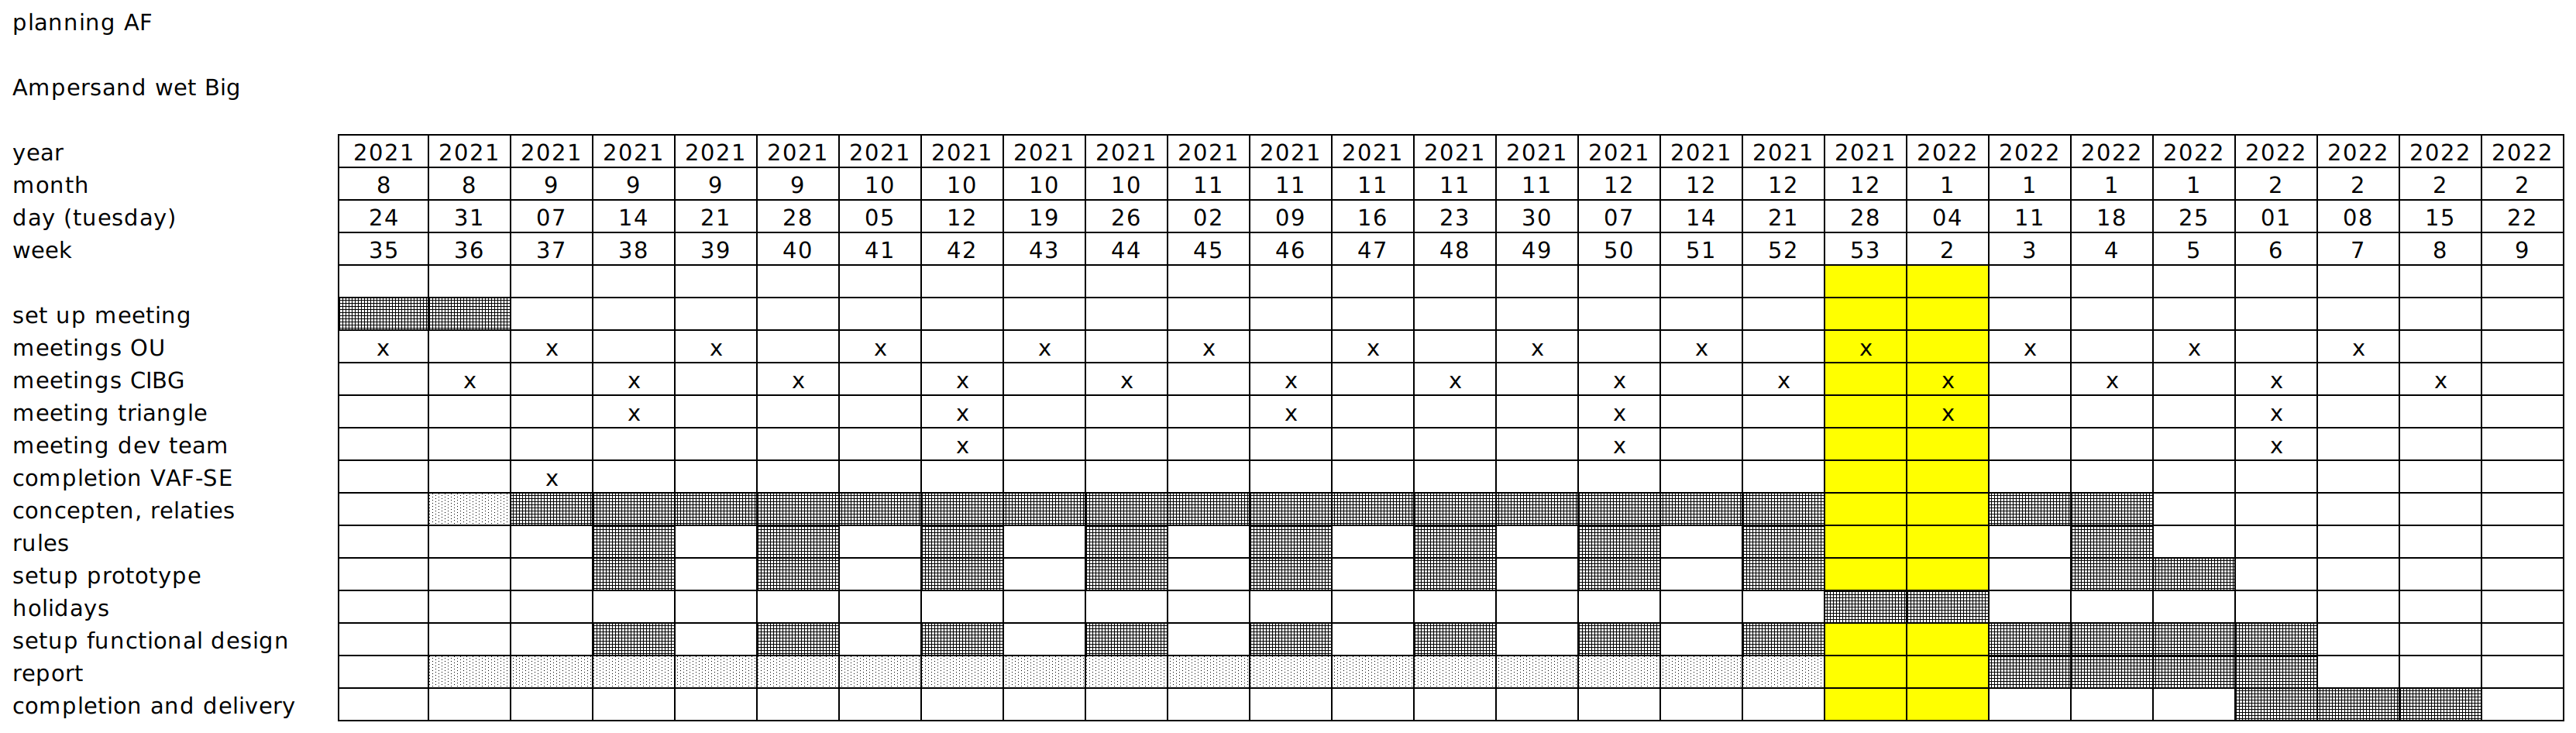
\includegraphics[width=1\textwidth]{00_common/04_images/planning.png}
    \caption{Planning}
    \label{fig:Planning}
\end{figure}
See the planning Figure~\ref{fig:Planning}
The Concepts, Relations and Rules must be continuously coordinated with the parties involved.
During the collection, the report is worked on so that the information collected during the process is a good reflection of the usefulness of Ampersand for analysing legislation and regulations.

\subsection{Risk analysis}
A short risk analysis
\begin{center}
\begin{tabular}{||l | l ||} 
 \hline
 \textbf{Risk} & \textbf{Possible action} \\ [0.5ex] 
 \hline\hline
 Not enough time to complete research & Time box approach; finish at the end of time \\ 
 \hline
 Outcome is not accepted & Explanation, finally acceptance \\
 \hline
 Illness and absence & Acceptance and yield less \\
 \hline
 Report not scientific enough & Adjust it to the required level \\
 \hline
 &   \\ [1ex] 
 \hline
\end{tabular}
\end{center}

